%%%%%%%%%%%%%%%%%%%%%%%%%%%%%%%%%%%%%%%%%%%%%%%%%%%%%%%%%%%%%%%%%%%%%%%%%%%%%%%%
%2345678901234567890123456789012345678901234567890123456789012345678901234567890
%        1         2         3         4         5         6         7         8

\documentclass[a4, 10 pt, conference]{ieeeconf}  % Comment this line out if you need a4paper

%\documentclass[a4paper, 10pt, conference]{ieeeconf}      % Use this line for a4 paper

\IEEEoverridecommandlockouts                              % This command is only needed if 
                                                          % you want to use the \thanks command

\overrideIEEEmargins                                      % Needed to meet printer requirements.

% See the \addtolength command later in the file to balance the column lengths
% on the last page of the document

% The following packages can be found on http:\\www.ctan.org
%\usepackage{graphics} % for pdf, bitmapped graphics files
%\usepackage{epsfig} % for postscript graphics files
%\usepackage{mathptmx} % assumes new font selection scheme installed
%\usepackage{times} % assumes new font selection scheme installed
%\usepackage{amsmath} % assumes amsmath package installed
%\usepackage{amssymb}  % assumes amsmath package installed
\usepackage{multicol}
\usepackage{tcolorbox}
\usepackage{cuted,tcolorbox,lipsum}
\usepackage{xcolor}
\usepackage{hyperref}
\usepackage{float}

\title{\LARGE \bf
Introduction to Machine Learning (SS 2024)\\ Programming Project
\vspace{-3em}
}


%\author{Fabio Plunser$^{1}$ and Dominik Barbist$^{2}$% <-this % stops a space
%}


\begin{document}


\maketitle
\vspace{-3em}
\thispagestyle{empty}
\pagestyle{empty}

\begin{strip}
  \begin{tcolorbox}[
      size=tight,
      colback=white,
      boxrule=0.2mm,
      left=3mm,right=3mm, top=3mm, bottom=1mm
    ]
    {\begin{multicols}{2}% replace 3 with 2 for 2 authors.

        \textbf{Author 1}       \\
        Last name: Plunser              \\  % Enter first name
        First name: Fabio             \\  % Enter first name
        Matrikel Nr.:               \\  % Enter Matrikel number

        \columnbreak

        \textbf{Author 2}       \\
        Last name: Barbist              \\  % Enter first name
        First name: Dominik             \\  % Enter first name
        Matrikel Nr.:               \\  % Enter Matrikel number

        \columnbreak

      \end{multicols}}
  \end{tcolorbox}
\end{strip}

%%%%%%%%%%%%%%%%%%%%%%%%%%%%%%%%%%%%%%%%%%%%%%%%%%%%%%%%%%%%%%%%%%%%%%%%%%%%%%%%

\section{Introduction}
\label{sec:intro}
We selected the Transaction dataset, which includes approximately 227,000 data points, each having 30 features (1 Time feature, 1 Amount feature, and 28 anonymized features). The dataset is labeled such that a transaction is
marked with a 1 if it is fraudulent and 0 if it is not, making the task a binary classification problem.

The dataset is highly imbalanced, with only about 0.001729\% of the data points labeled as fraudulent. This extreme imbalance poses a significant challenge for the classification task, as the model may become
biased towards predicting the majority class (non-fraudulent transactions).

The 28 other features are anonymized, and their exact meanings are unknown. However, these features do not contain any missing values.

\section{Implementation / ML Process}
\label{sec:methods}

% {\color{blue}

%   \begin{itemize}
%     \item Did you need to pre-process the dataset (e.g. augmenting data points, extracting features, reducing the dimensionality, etc.)? If so, describe how you did this.
%     \item Specify the method (e.g. linear regression, or neural network, etc.). You do not have to describe the algorithm in detail, but rather the algorithm family and the properties of the algorithm within that family, e.g. which distance functions for a decision tree, what architecture (layers and activations) for a neural network, etc.
%     \item State (in 2-5 lines) what makes the algorithm you chose suitable for this problem. What are the reasons for choosing your ML method over others?
%     \item If you used a method that was not covered in the VO, describe how it is different from the closest method described in the VO.
%     \item How did you choose hyperparameters (other design choices) and what are the values of the hyperparameters you chose for your final model? How did you make sure that the choice of hyperparameters works well?
%   \end{itemize}
% }

\subsection{Preprocessing}
\label{sec:preprocess}
Due to the imbalanced nature of the dataset, we employed an oversampling technique to balance the classes. We used a custom
oversampling function that generates synthetic samples for the minority class (fraudulent transactions) based on the k-nearest
neighbors algorithm. This approach involves generating new fraudulent samples by interpolating between existing fraudulent
samples and their nearest neighbors.

\subsection{Logistic Regression}
Logistic regression is one of the most straightforward classification algorithms, making it a suitable initial approach for binary classification tasks.
This model estimates the probability that a given input belongs to a particular class using a logistic function.

\subsubsection{Hyperparameters}
We use completely standard hyperparameters without any fine tuning.
We tried some different solvers and maximumt iterations but the outcome didn't change much.
The hyperparameters we used are:
Solver: lbfgs, Max iterations: 100
The biggest impact on the performance was the oversampling.

\subsubsection{Model Description}
Logistic regression operates by applying the logistic function to a linear combination of input features, yielding a probability score between 0 and 1.
This probability is then used to classify the input into one of the two classes. Given its simplicity and ease of implementation, logistic regression serves
as an effective starting point for classification problems.

\subsection{Neural Network(MLP)}
MLPs are a class of feedforward neural networks that consist of multiple layers of neurons, each layer fully connected to the next. With the ability to learn complex patterns
in the data, MLPs are well-suited for classification tasks. Espacially for the given dataset, which has 30 features, a neural network can learn the complex patterns in the data and classify the data into the two classes.

\subsubsection{Hyperparameters}
For the neural network model, we used 3 hidden layers with 256 neurons each, and a initial learning rate of 0.0001. We trained the model for 40 epochs with a batch size of 128.

\subsubsection{Model Description}
In our neural network model, we used a learning rate optimization techniques(e.g. scheudler). The learning rate scheduler is used to adjust the learning rate during training,
which can speed up the training process and improve the model's performance. We used a early stopping to stop the training process when the model's performance stops improving.

\section{Results}
\label{sec:results}

% {\color{blue}

%   \begin{itemize}
%     \item Describe the performance of your model (in terms of the metrics for your dataset) on the training and validation sets with the help of plots or/and tables.
%     \item You must provide at least two separate visualizations
%           (plot or tables) of different things, i.e. don’t use a table
%           and a bar plot of the same metrics. At least three
%           visualizations are required for the 3 person team.
%   \end{itemize}
% }

Scores with validation set
\begin{center}
  \begin{table}[!h]
    \resizebox{0.45\textwidth}{!}{
      \begin{tabular}{l|c|c|c|c|c}
        Model               & Accuracy & Precision & Recall   & F1-Score & ROC-AUC  \\\hline
        Logistic Regression & $0.9990$ & $0.9990$  & $0.9984$ & $0.9986$ & $0.9486$ \\\hline
        Neural Network      & $0.9989$ & $0.9991$  & $0.9989$ & $0.9990$ & $0.9237$ \\
      \end{tabular}
    }

  \end{table}
\end{center}


\subsection{Logistic Regression}
\begin{figure}[H]
  \centering
  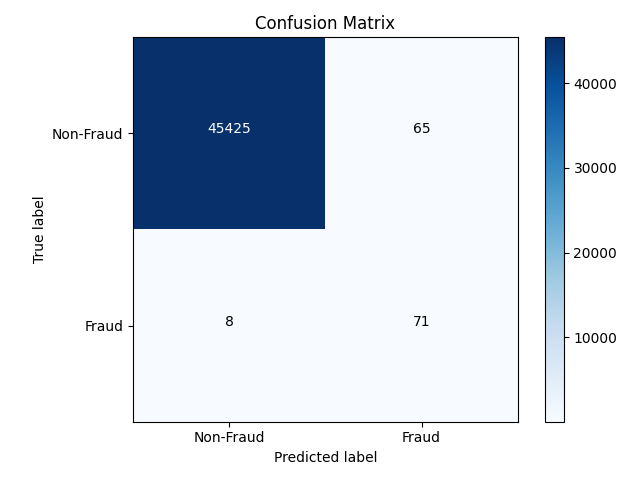
\includegraphics[width=0.35\textwidth]{images/confusion_matrix.png}
  \caption{Conusion Matrix}
  \label{fig:lr-confusion}
\end{figure}
As you can see in the confusion matrix \ref{fig:lr-confusion} the model predicts 94\% of all fraud cases correctly and only has a false positive rate of 0.1431\%.

\begin{figure}[!htb]
  \centering
  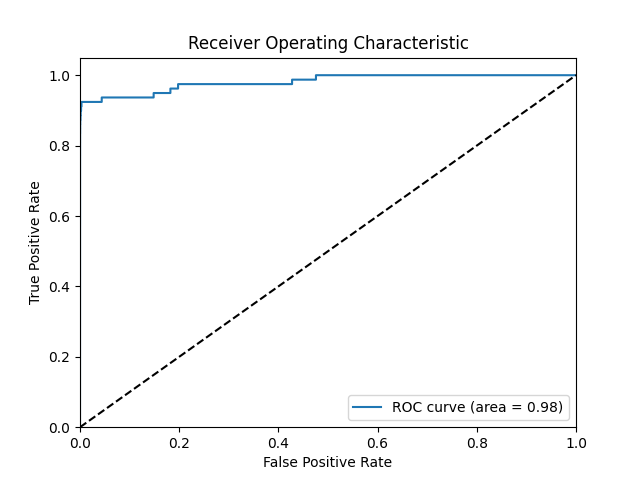
\includegraphics[width=0.35\textwidth]{images/roc_curve.png}
  \caption{ROC-Curve}
  \label{fig:lr-roc}
\end{figure}
% The ROC () curve is a graphical representation of a classifier's performance across all classification thresholds.
% It plots the True Positive Rate (sensitivity) against the False Positive Rate (1-specificity).
% The area under the ROC curve (AUC) is a measure of the model's ability to distinguish between classes, with an AUC of 1.0 representing a perfect classifier.
In the provided ROC curve \ref{fig:lr-roc}, the model demonstrates a high performance with an AUC of 0.98, indicating excellent discrimination ability.

\subsection{Neural Network}
\begin{figure}[!htb]
  \centering
  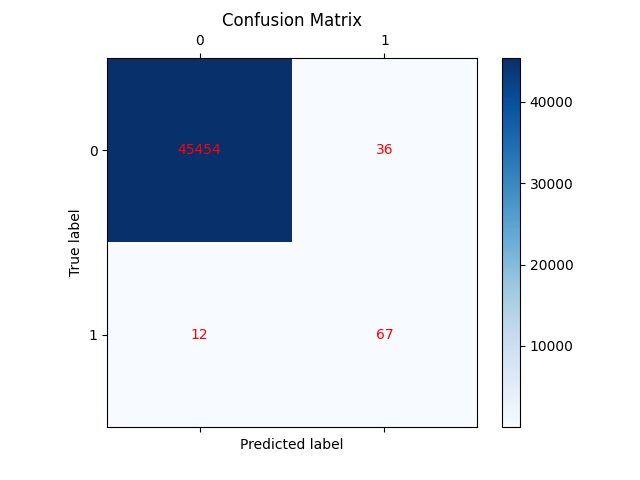
\includegraphics[width=0.35\textwidth]{images/ml_confusion.png}
  \caption{Confusion Matrix}
  \label{fig:ml-confusion}
\end{figure}
As you can see in the confusion matrix \ref{fig:ml-confusion} is quite similar to the confusion matrix of the logistic regression model.
\begin{figure}[!htb]
  \centering
  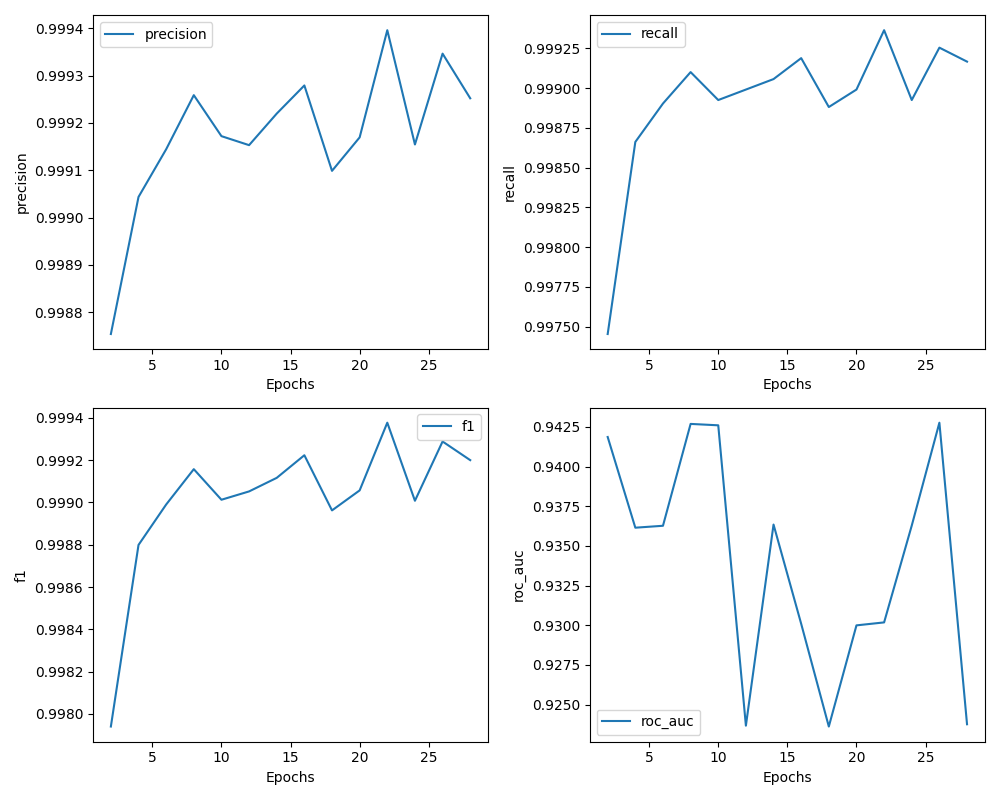
\includegraphics[width=0.35\textwidth]{images/ml.png}
  \caption{ML-Metrics}
  \label{fig:ml}
\end{figure}
As you can see over time the model gets better and better, in each metric. With some more epochs, and fine tuning of the hyperparameters, the model could achieve even better results.


\section{Discussion}
\label{sec:discuss}

% {\color{blue}
%   \begin{itemize}
%     \item Analyze the results presented in the report (comment on what contributed to the good or bad results). If your method does not work well, try to analyze why this is the case.
%     \item Describe very briefly what you tried but did not keep for your final implementation (e.g. things you tried but that did not work, discarded ideas, etc.).
%     \item How could you try to improve your results? What else would you want to try?

%   \end{itemize}
% }

The results of both models are quite good, with all the metrics being above 0.95\%. Over all the main bottleneck of the project was the imbalanced dataset. The oversampling technique helped to improve the results of the models. But thoese data are still only synthetic data and can't replace real data.
For the neural network model, we try to use some additional methods to prevent overfitting(e.g. dropout, and weight decay), which we discarded in the final implementation. For the logistic regression model, we tried some different solvers and maximum iterations, but the outcome didn't change much.

\subsection{Choice}
Both of the models show similar results when it comes to classify give data into the two classes. The logistic regression model is easier to implement and faster to train. The neural network model is more complex and takes longer to train. The neural network model has more hyperparameters to tune, which can lead to better results if tuned correctly.
The logistic regression model is a good starting point for binary classification tasks, and the neural network model is a more advanced model that can achieve better results with the right hyperparameters. So we decided to use the logistic regression model as our Model for the final implementation.

\section{Conclusion}
\label{sec:con}

% {\color{blue}

%   \begin{itemize}
%     \item Finally, describe the test-set performance you achieved. Do not
%           optimize your method based on the test set performance!
%     \item Write a 5-10 line paragraph describing the main takeaway of your project.
%   \end{itemize}

% }

\begin{center}
  \begin{table}[!h]
    \resizebox{0.45\textwidth}{!}{
      \begin{tabular}{l|c|c|c|c|c}
        Model               & Train Dataset Score & Test Dataset Score \\\hline
        Logistic Regression & $0.5888$            & $0.5625$           \\\hline
        Neural Network      & $0.5873$            & $0.5595$           \\
      \end{tabular}
    }

  \end{table}
\end{center}
In this project, we explored the performance of two machine learning models—Logistic Regression and a Neural Network—on a highly imbalanced transaction dataset aimed at detecting fraudulent transactions.
Both models have very simular results, with the new data the logistic regression is marginally better. 
The logistic regression model is a good starting point for binary classification tasks, 
while the neural network model is a more advanced model that could achieve better results with the right hyperparameters.
%%%%%%%%%%%%%%%%%%%%%%%%%%%%%%%%%%%%%%%%%%%%%%%%%%%%%%%%%%%%%%%%%%%%%%%%%%%%%%%%
\end{document}
